\section{Mote Harness}

In order to guarantee that both sender and receiver will not move during experiments a plexiglass harness was developed.
The mote snaps into the harness which then allows rotation of the PCB antenna around the z-axis in 5$^\circ$ steps.
A top view vector drawing of the rotation dish is shown in Figure~\ref{fig:harness_vector}.

Furthermore, the distance between two harnesses can be adjusted in 5mm steps using laser-cut wooden distance bars as shown in Picture~\ref{pic:harness_distance}

\begin{figure}[H]
	\centering
    % \includegraphics[trim = 5mm 5mm 140mm 25mm, clip, width=1\columnwidth, angle=90, scale=0.5]{figures/harness_vector}
    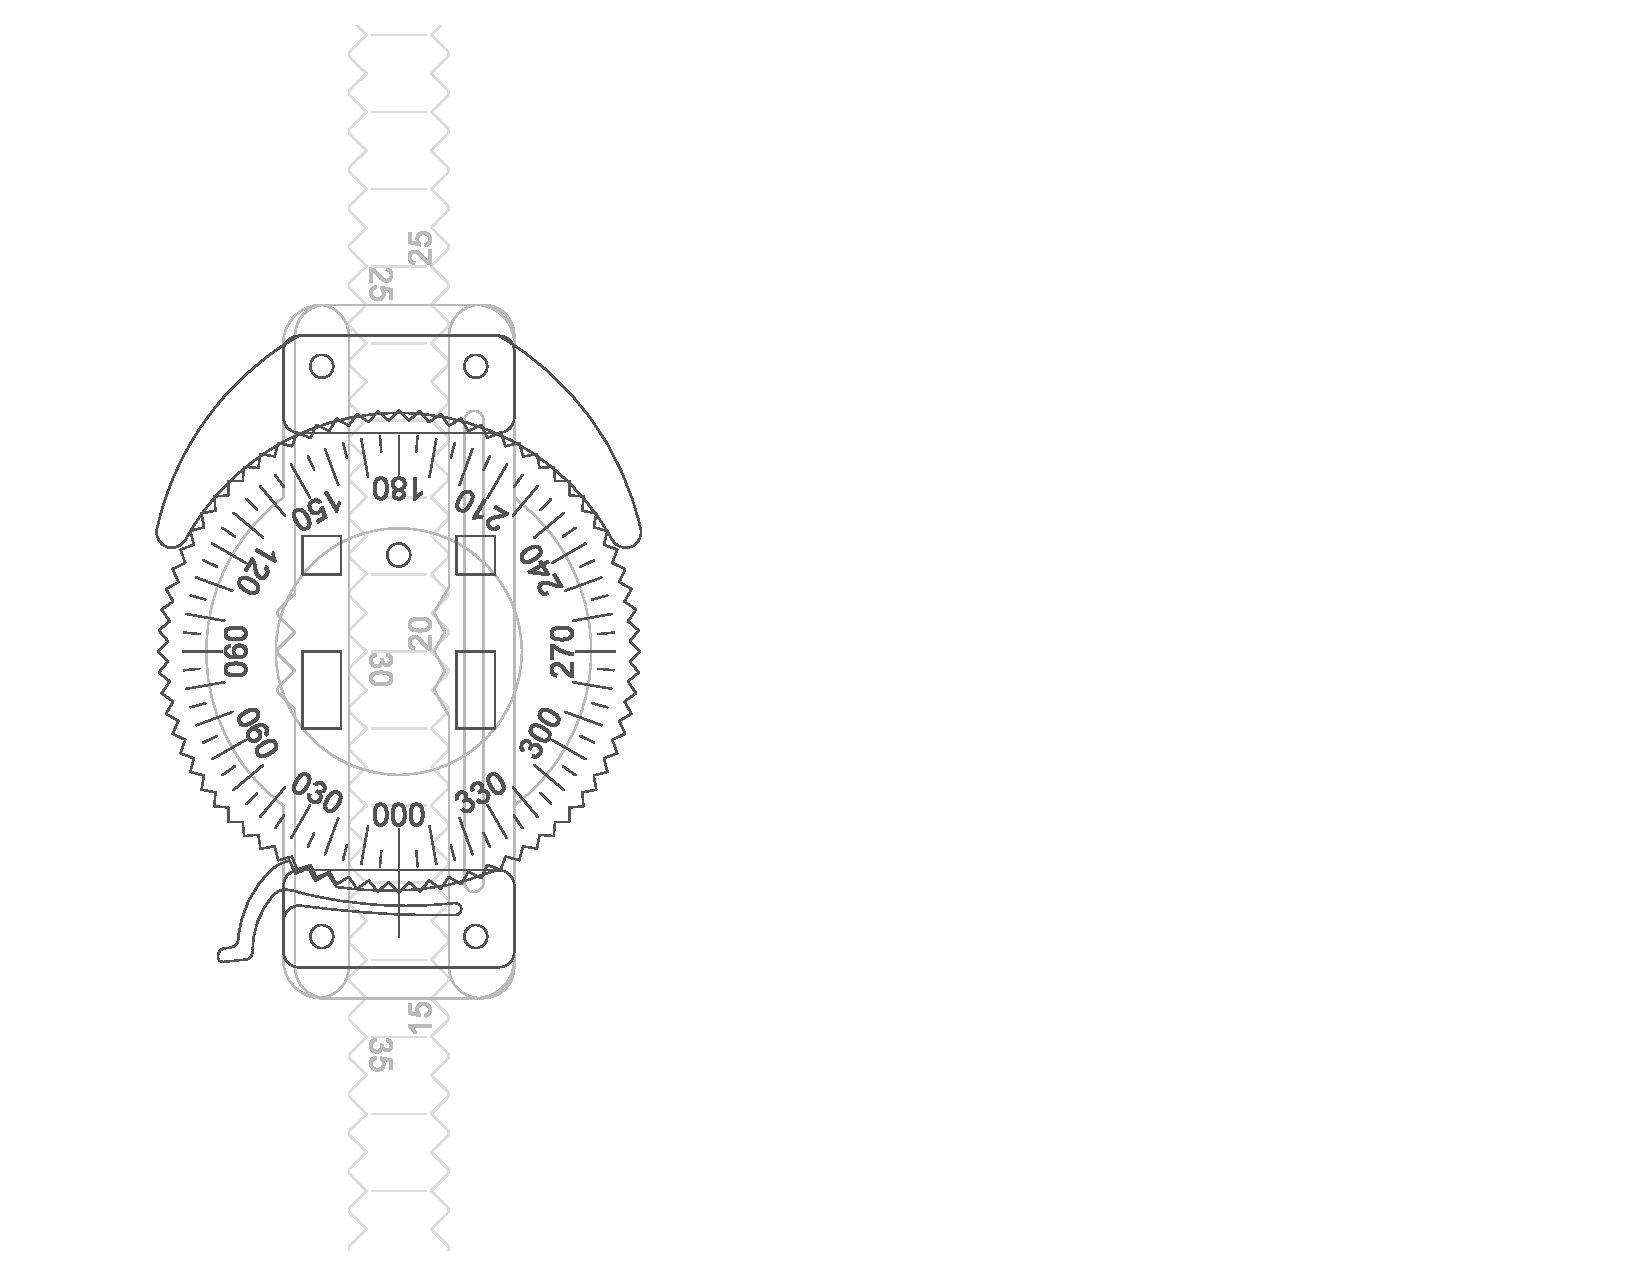
\includegraphics[trim = 20mm 20mm 120mm 25mm, clip, width=1\columnwidth, angle=90, scale=0.75]{figures/harness_vector_bar_2}
	\caption{The rotation dish and distance bars (mote and harness not depicted for clarity).}
    \label{fig:harness_vector}
\end{figure}

In our experiments changing PCB antenna orientation had a much higher impact on link quality than increasing or decreasing distance between two motes.
As shown in Figure~\ref{fig:antenna_orientation_lqi}, the changes in LQI is quite dramatic even with small (5) changes to antenna orientation.
